\section{Testing Environment and Method}
The automated tests were executed on 20 June 2026 with Node.js 22.12.0 using the built-in Node test runner and experimental coverage instrumentation. The command was:

\begin{Verbatim}[fontsize=\small,frame=single]
node --test --experimental-test-coverage \
  test/focusMetrics.test.js test/firestoreModels.test.js
\end{Verbatim}

The two suites focus on deterministic business logic that can be validated without external services. This was important because the current prototype depends on Google authentication, Firestore, Expo web/mobile runtime behaviour, and camera permissions. Those dependencies are valuable for end-to-end validation, but they make low-level regression tests slower and harder to run consistently.

\texttt{focusMetrics.test.js} covers time formatting, invalid-value clamping, daily and total statistics, progress limits, session payloads, ISO date normalization, and elapsed-minute calculation. These tests protect the Focus Timer and Dashboard logic.

\texttt{firestoreModels.test.js} covers snapshot mapping, profile and session payloads, participant defaults, room normalization, active-room filtering, and rejection of unavailable rooms. These tests protect the data-shaping rules used before writing to Firestore and after reading Firestore snapshots, without touching the real cloud database.

\begin{figure}[H]
\centering
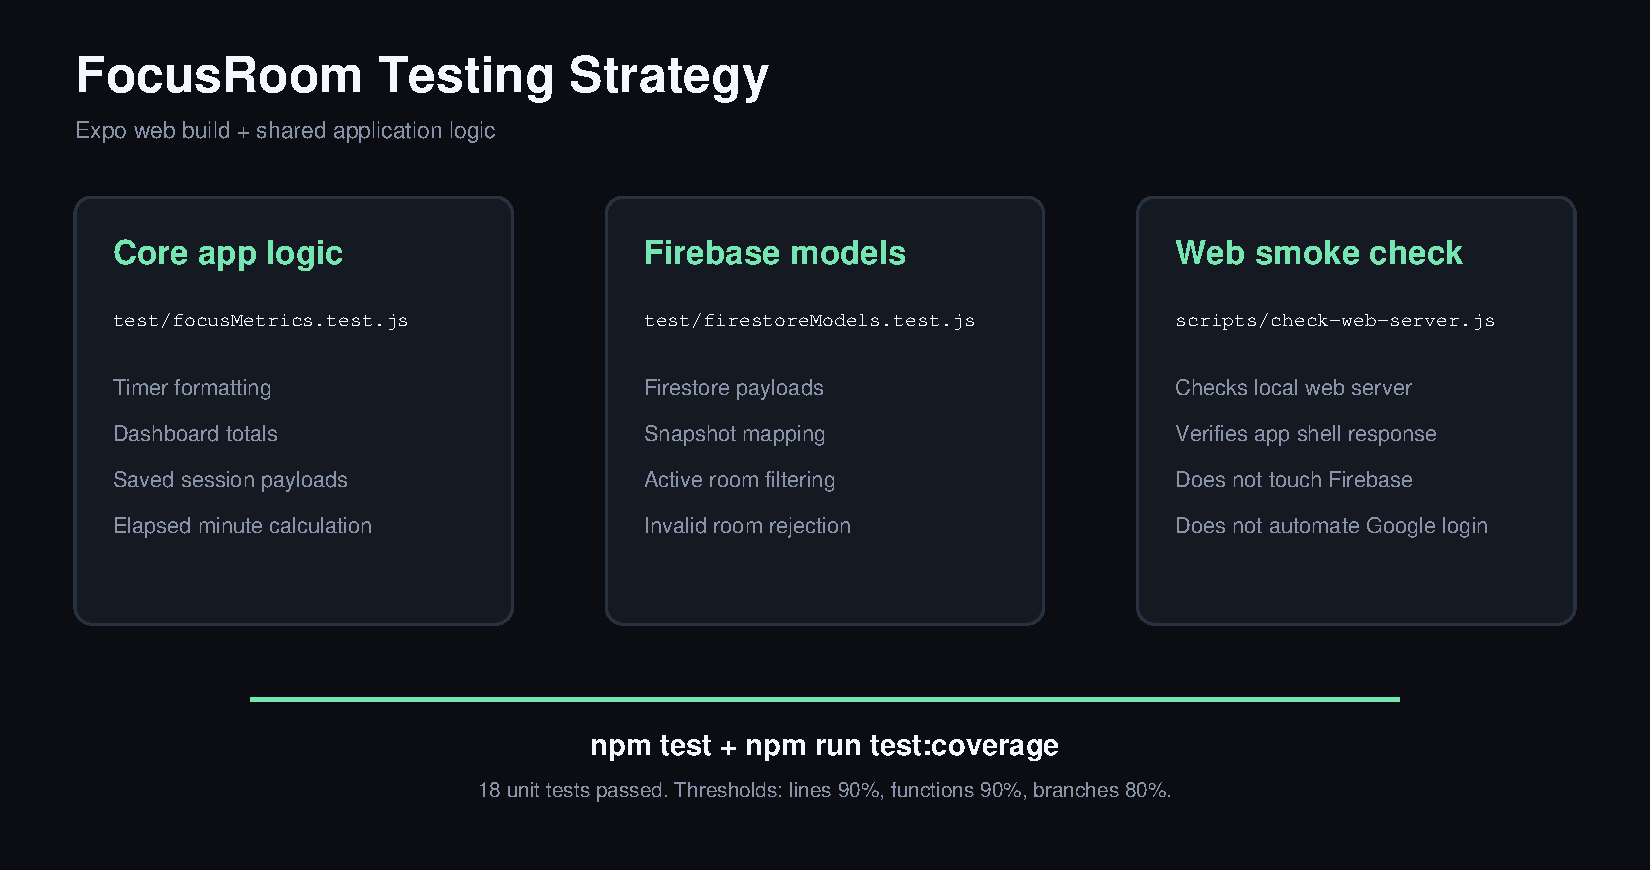
\includegraphics[width=0.95\textwidth]{Images/testing-strategy.pdf}
\caption{Testing strategy for the FocusRoom web prototype}
\label{fig:testing_strategy}
\end{figure}

\section{Results}
All 18 test cases passed. No tests were skipped or cancelled. The observed test-runner duration was 144.99 ms in the final verification run.

\begin{table}[H]
\centering
\begin{tabular}{|l|r|}
\hline
\textbf{Metric} & \textbf{Result} \\ \hline
Test files & 2 \\ \hline
Test cases & 18 \\ \hline
Passed & 18 \\ \hline
Failed & 0 \\ \hline
Skipped / cancelled & 0 \\ \hline
Pass rate & 100\% \\ \hline
\end{tabular}
\caption{Automated test results}
\label{tab:test_results}
\end{table}

The tests are grouped as follows:

\begin{itemize}
  \item \textbf{Core application logic:} verifies timer formatting, dashboard aggregation, daily goal progress, saved-session payload generation, and elapsed-minute calculation.
  \item \textbf{Firebase data models:} verifies Firestore payload construction, document snapshot mapping, participant defaults, active-room filtering, and unavailable-room rejection.
  \item \textbf{Web smoke check:} verifies that the local Expo web server can return the FocusRoom app shell. This check is intentionally lightweight and does not automate Google login or Firebase data inspection.
\end{itemize}

\section{Coverage}
\begin{table}[H]
\centering
\begin{tabular}{|l|r|r|r|}
\hline
\textbf{Source file} & \textbf{Lines} & \textbf{Branches} & \textbf{Functions} \\ \hline
\texttt{firestoreModels.js} & 100.00\% & 93.75\% & 100.00\% \\ \hline
\texttt{focusMetrics.js} & 100.00\% & 82.35\% & 100.00\% \\ \hline
\textbf{Overall} & \textbf{100.00\%} & \textbf{87.88\%} & \textbf{100.00\%} \\ \hline
\end{tabular}
\caption{Coverage of tested production modules}
\label{tab:coverage}
\end{table}

\begin{figure}[H]
\centering
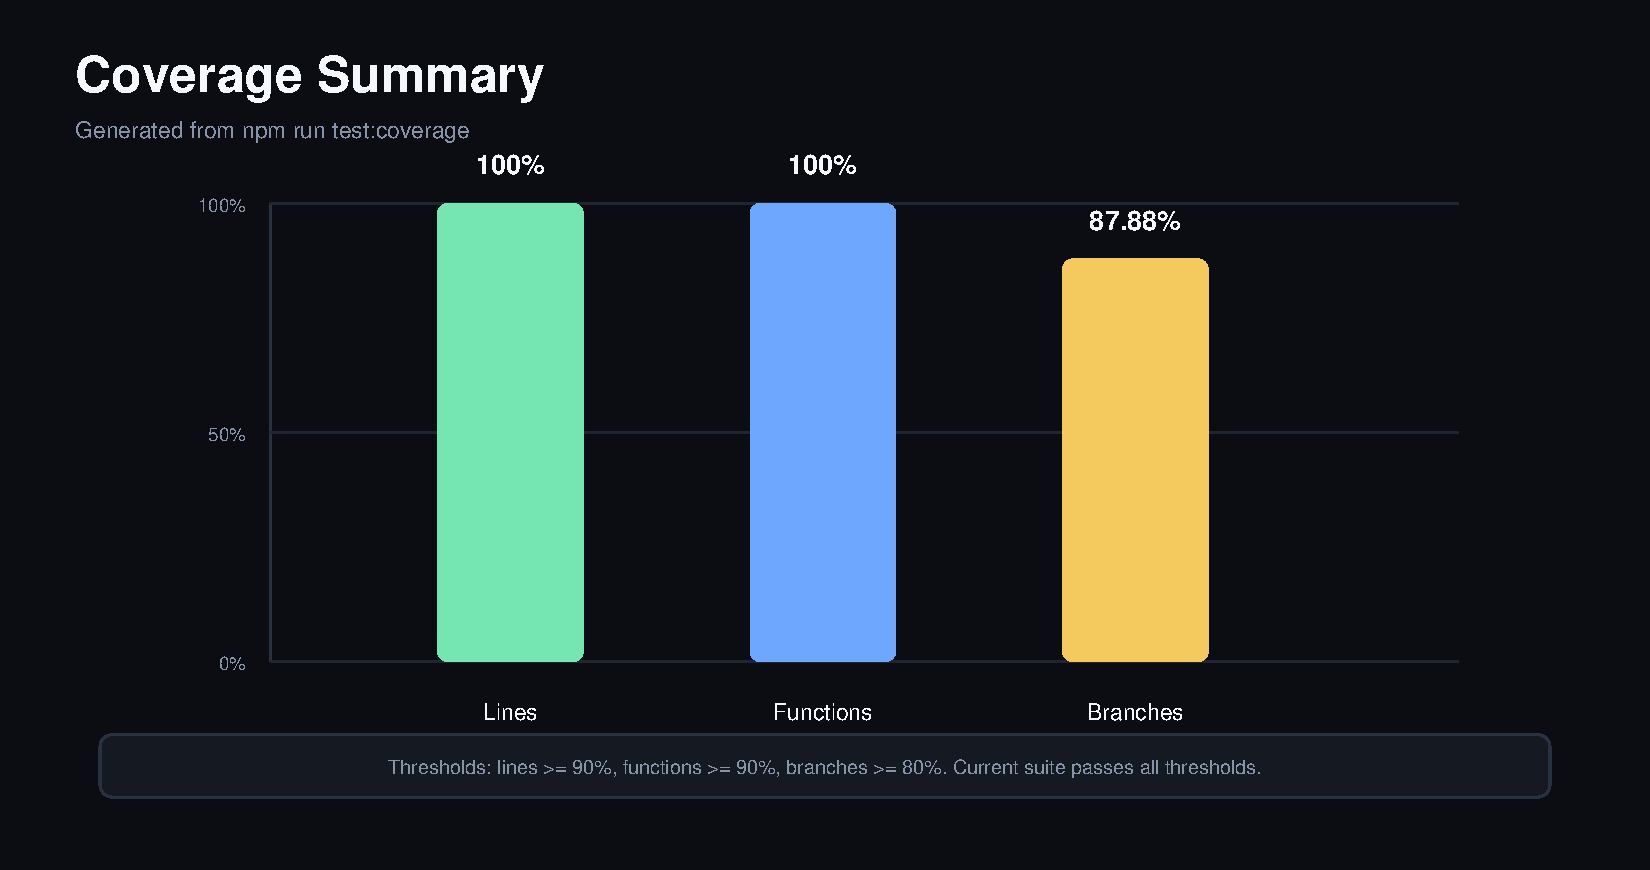
\includegraphics[width=0.9\textwidth]{Images/coverage-summary.pdf}
\caption{Coverage summary for tested utility modules}
\label{fig:coverage_summary}
\end{figure}

The results provide strong evidence for the extracted mapping and calculation functions, but they do not establish end-to-end correctness of the distributed application. Authentication providers, Firestore transactions and rules, camera permissions, token issuance, WebRTC connections, reconnection behavior, and UI interaction remain outside the automated suite.

\section{Error Handling and Edge Cases}
The current tests cover several important edge cases in the shared logic layer:

\begin{itemize}
  \item Negative or invalid timer values are clamped to \texttt{00:00}.
  \item Empty session lists produce zeroed dashboard statistics.
  \item Daily goal progress is capped at \texttt{100\%}.
  \item Elapsed focus sessions save at least one minute.
  \item Missing Google profile fields fall back to safe empty values.
  \item Missing participant names fall back to \texttt{Student}.
  \item Rooms marked with \texttt{active === false} are removed from the available-room list.
  \item Missing or inactive room snapshots are rejected before joining.
\end{itemize}

\section{Recommended Validation Campaign}
The next validation layer should use the Firebase Emulator Suite to exercise authorization rules and room/session write paths. Integration tests should verify Google sign-in success, cancellation, and failure states using a controlled test account or mocked authentication boundary. Device testing should cover camera denial, backgrounding during a focus session, network handover, reconnection behavior, and mixed web/native participants. Finally, end-to-end flows should verify that focus and room sessions appear correctly in the Dashboard after being created from another device.

For the current repository, the relevant test files are:

\begin{itemize}
  \item \texttt{test/focusMetrics.test.js}
  \item \texttt{test/firestoreModels.test.js}
  \item \texttt{src/utils/focusMetrics.js}
  \item \texttt{src/utils/firestoreModels.js}
  \item \texttt{scripts/check-web-server.js}
\end{itemize}
